\nonstopmode
\documentclass[12 pt, a4paper]{article}
\usepackage[warn]{ mathtext }
\usepackage[utf8]{inputenc} 
\usepackage[russian,english]{babel}
\usepackage[T1, T2A]{fontenc}
\usepackage{graphicx}
\usepackage{minted}
\usepackage[left=2cm,right=2cm,top=2cm,bottom=2cm,bindingoffset=0cm]{geometry}
\graphicspath{ {images/} }
\title{\textbf{Санкт-Петербургский государственный университет \\
Математико-механический факультет} \vspace{6cm} \\ Базы данных и СУБД \\
Отчёт по самостоятельному заданию\vspace{6cm}}
\author{Студент: Овсянников К. А., гр. 22Б-10 ММ }
\date{весна 2024 г.}
\begin{document}
\maketitle
\newpage
\section{Описание предметной области}
\subsection{Требования заказчика}
Компания-заказчик занимается продажей и ремонтом авто- и мототехники. Реализация осуществляется в отделениях, расположенных по всей стране. Также компания имеет сеть сервисов, которые занимаются ремонтом и обслуживанием техники. В каждом из сервисов работают опытные специалисты, осуществляющие ремонт техники определённых типов и марок.\\
Расчёт стоимости за услугу осуществляется из базовой цены услуги и умножающего коэффициента соответствующего конкретной модели техники.\\
Требуется создать базу данных для учёта имеющихся в наличии ТС, контроля зарплат сотрудников и отображения набора услуг.\\
\subsection{ER-диаграмма}
\begin{center}
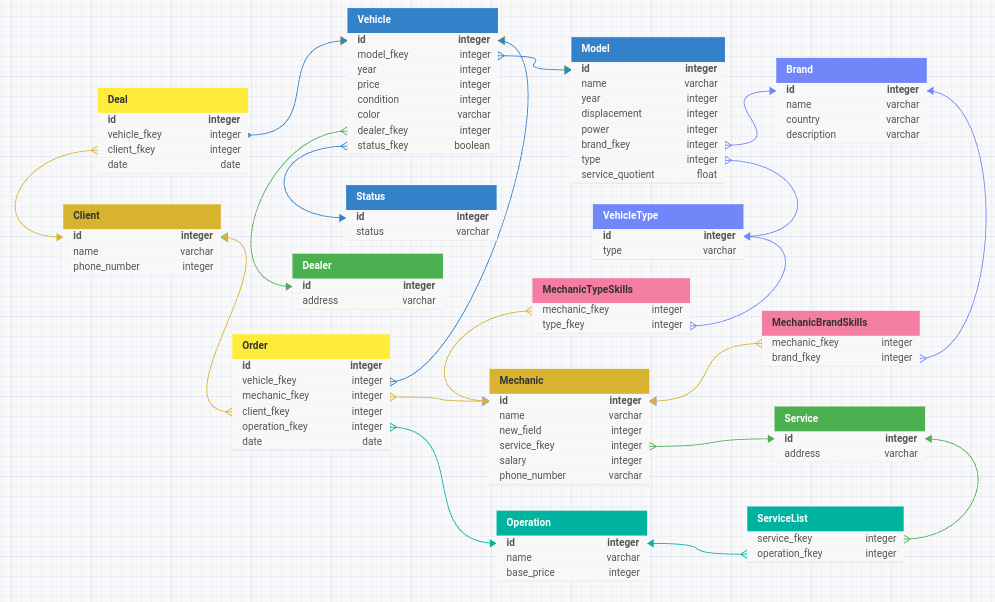
\includegraphics[scale=0.62]{er.png}
\end{center}
\section{Скрипты}
\subsection{Скрипт создания таблиц и ограничений в базе данных}
\inputminted{sql}{ololo.sql}
\inputminted{sql}{../scripts/create_db.sql}
\subsection{Скрипт заполнения базы данных}
\inputminted{sql}{../scripts/fill_db.sql}
\subsection{Скрипт удаления всех таблиц в базe данных}
\inputminted{sql}{../scripts/drop_db.sql}
\subsection{Скрипт очистки всех таблиц в базе данных}
\inputminted{sql}{../scripts/clear_db.sql}
\subsection{Пользовательские запросы}
\subsection{Процедуры}
\subsubsection{Статистические функции}
\inputminted{sql}{../scripts/statistic_functions.sql}
\subsection{Триггеры}
\inputminted{sql}{../scripts/triggers.sql}
\subsection{Представления}
\end{document}

